
                        \documentclass{article}
                        \usepackage{tikz}
                        \usetikzlibrary{automata, positioning}

                        \begin{document}
                        \section{}

                            \begin{center}
                                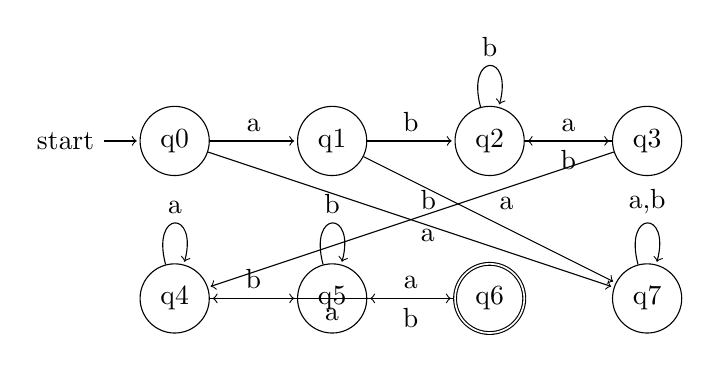
\begin{tikzpicture}[shorten >=1pt, node distance=2cm, on grid, auto] 
                    
    \node [state,initial] (q0) at (0 , 0) { q0};
    \node [state] (q1) at (2 , 0) { q1};
    \node [state] (q2) at (4 , 0) { q2};
    \node [state] (q3) at (6 , 0) { q3};
    \node [state] (q4) at (0 , -2) { q4};
    \node [state] (q5) at (2 , -2) { q5};
    \node [state,accepting] (q6) at (4 , -2) { q6};
    \node [state] (q7) at (6 , -2) { q7};
 \path[->]
      (q0) edge node {a} (q1)
      (q0) edge node {b} (q7)
      (q1) edge node {a} (q7)
      (q1) edge node {b} (q2)
      (q2) edge node {a} (q3)
      (q2) edge[loop above] node {b} (q2)
      (q3) edge node {a} (q4)
      (q3) edge node {b} (q2)
      (q4) edge node {b} (q5)
      (q4) edge[loop above] node {a} (q5)
      (q5) edge node {a} (q6)
      (q5) edge[loop above] node {b} (q5)
      (q6) edge node {a} (q4)
      (q6) edge node {b} (q5)
      (q7) edge[loop above] node {a,b} (q7);
                        \end{tikzpicture}
                        \end{center}
                        \end{document}
                        